	\begin{theorem} \label{thm: commuting connecting homomorphism}
	Given the filtration $N_{-1}\subseteq N_0 \subseteq \cdots \subseteq N_{m-1} \subseteq N_m=M$   from (\ref{eq: Filtration conley}).  The following diagram commutes:
	\begin{center}
		% https://tikzcd.yichuanshen.de/#N4Igdg9gJgpgziAXAbVABwnAlgFyxMJZABgBpiBdUkANwEMAbAVxiRAGEA9YAawF8AFAFlSAHVEBbOjgAWAMwBOdHsACCfMaLwNYwANJ9uDQWhwBKMyA3pMufIRQBGclVqMWbLrwDUjwSPEpWUVlNQ1xbV0DIxNzS2sQDGw8AiIyR1d6ZlZEEHEAIywAcwg0ZjhxBiwJXDgAfWA0cSwwAAJxdgVcOp4BOTM+fUMfYwEAOTq0UgAZSfjSG2T7ImcM6iyPXILi0vLK6tqGgEdmto6unAaeX0F+weiRm-G6o5mX+cW7VJQyACZM9w5EB6bjXUYTHikCa8AC0fg+iVsKQcyGc-3WgLYIMa3gYT2h1z8UJ68VcMCgRXgRFAiggEiQZBAOAgSGcbmybHEaDoCjwjE4aCsCxAtPpiEZzKQvwSotZ1EliAAzDKFHSkAAWeUsxAAVgxHK2olgDBwdAaOC6ZRgfCFNNVYt+Wo1KrVSqdupdDvdiv1mzyogAIjATWaRja+BQ+EA
		\begin{tikzcd}
			{C^{k}(M,\mathfrak{A},\tilde{K}^{l}(pt))} \arrow[r, "\partial^p"] \arrow[d]                & {C^{k+1}(M,\mathfrak{A},\tilde{K}^{l}(pt))} \arrow[d]                  \\
			{\bigoplus\limits_{p\in \Crit_k(f)}{K}^{k+l}(N_p,L_p)} \arrow[d] \arrow[r, "\Delta_{k+l}"] & {\bigoplus\limits_{q\in \Crit_{k+1}(f)}{K}^{k+l+1}(N_q,L_q)} \arrow[d] \\
			{K^{k+l}(N_k,N_{k-1})} \arrow[r, "\delta_{triple}"]                                        & {K^{p+l+1}(N_{k+1},N_k)}                                              
		\end{tikzcd}
	\end{center}
\end{theorem}
\begin{Iprove}
	We will first build up a diagramm that encapusates the connecting homomorphism from K-theory, which was build as follows: Assume that $(X,Y,Z)$ is a topological triple. Then the first map is induced from the kollaps: $Y\to Y\big/ Z$. Afterwards we have the connecting homomorphism of the pair $(X,Y)$:
	
	The K-groups of the pointed spaces $X\big/ Y$ and $X\cup CY$, where the latter denotes a cone above $Y$ agree. From the latter we can quotien out $X$, and $X\cup CY\big/ X\cong SY$. Hence we have the triple connecting homomophism as the composition:
	\begin{equation*}
		K^{-1}(Y,Z)\to	K^{-1}(Y)=K(SY)\cong K(X\cup CY\big/ X)\to K(X\cup CY)\cong K(X\big/ Y) 
	\end{equation*}The triple connecting homomorphism for lower K-Groups is defined exactly the same via the identification $K^{-n}(X,Y)=K(S^n\vee (X,Y))$. For higher K-Groups we apply the natural Bott isomorphism and make use of the identity. By doing this we get the tripple homomorphism 
	\begin{center}
		% https://tikzcd.yichuanshen.de/#N4Igdg9gJgpgziAXAbVABwnAlgFyxMJZABgBpiBdUkANwEMAbAVxiRAGkA9MACgE1SALQCUIAL6l0mXPkIoyARiq1GLNl2ABaMGP5DREqdjwEiC0kur1mrRB05adetAckgMx2UQBMF5dbU7DW0AagVdAA1SPlcjGVMUAGY-K1Vbe0dNcJ4omPE3D3i5ZGTKVJt1BzAwyOiDZRgoAHN4IlAAMwAnCABbJDIQHAgkcxAGLDB0qAgmACMGVmoACxg6KDZISZBqHDosBg2CVkMQLt6RneHEXxUKuyxOACp8ju6+68ukZNvAkAAdP6wBi7AD6wGmcwWYhepzeX0+iAALOVfrMIDgcDCzu8AKwI5FjCZTGbzRYgFZrQ5bHZ7A52TbHNzY-oIvE-dIAoGg4A4TpYNBQ8QUMRAA
		\begin{tikzcd}
			{K^n(Y,Z)} \arrow[d, no head, Rightarrow] \arrow[rrr, "\delta_{triple}"] &                                            &                                   & {K^{n+1}(X,Y)} \arrow[d, no head, Rightarrow] \\
			{K^{-n}(Y,Z)} \arrow[r, "i^*"]                                           & {K^{-n}(Y,p)} \arrow[r, "\delta_{double}"] & {K^{-n+1}(X,Y)} \arrow[r, "bott"] & {K^{-n-1}(X,Y)}                              
		\end{tikzcd}
	\end{center} For the proof of the upper square, we actually proof that the following commutes:
	\begin{fdiagram}\label{diag: that we really want to show}
		% https://tikzcd.yichuanshen.de/#N4Igdg9gJgpgziAXAbVABwnAlgFyxMJZABgBpiBdUkANwEMAbAVxiRAGEA9YAawF8AFAFlSAHVEBbOjgAWAMwBOdHsACCfMaLwNYwANJ9uDQWhwBKMyA3pMufIRQBGclVqMWbLrwDUjwSPEpWUVlNQ1xbV0DIxNzS2sQDGw8AiIyR1d6ZlZEEHEAIywAcwg0ZjhxBiwJXDgAfWA0cSwwAAJxdgVcOp4BOTM+fUNgAFp+AQA5OrRSABlp+NIbZPsiZwzqLI9cguLS8srq2oaAR2a2jq6cBp5fQX7B6NGBW8cBybqTuc-41xgoIrwIigRQQCRIMggHAQJDONzZNjiNB0BR4RicNBWJYgUHgxCQ6FIABMCVxsOohMQAGZSQowcSKTDqZt3Dk8qIACIwBg4Og3PhWCh8IA
		\begin{tikzcd}
			{C^{k}(M,\mathfrak{A},\tilde{K}^{l}(pt))} \arrow[r, "\partial^p"] \arrow[d]   & {C^{k+1}(M,\mathfrak{A},\tilde{K}^{l}(pt))} \arrow[d]         \\
			{\bigoplus\limits_{p\in \Crit_k(f)}{K}^{-k}(N_p,L_p)} \arrow[r, "\Delta_{k}"] & {\bigoplus\limits_{q\in \Crit_{k+1}(f)}{K}^{-(k+1)}(N_q,L_q)}
		\end{tikzcd}
	\end{fdiagram}
	Furthermore we assumed that $l=0$. This doesnt change the generality since if $l$ was even, we can apply the Bott isomorphism and else the groups are $0$. 
	Now we choose a triple $(A,B,C)$ in $M$ such that: 
	\begin{enumerate}[(a)]
		\item $(A,B)$ is a regular index pair for a critical point $q\in \Crit_{k+1}\,$.
		\item $(B,C)$ is a regular index pair for a critical point $p\in \Crit_{k}\,$.
	\end{enumerate}
	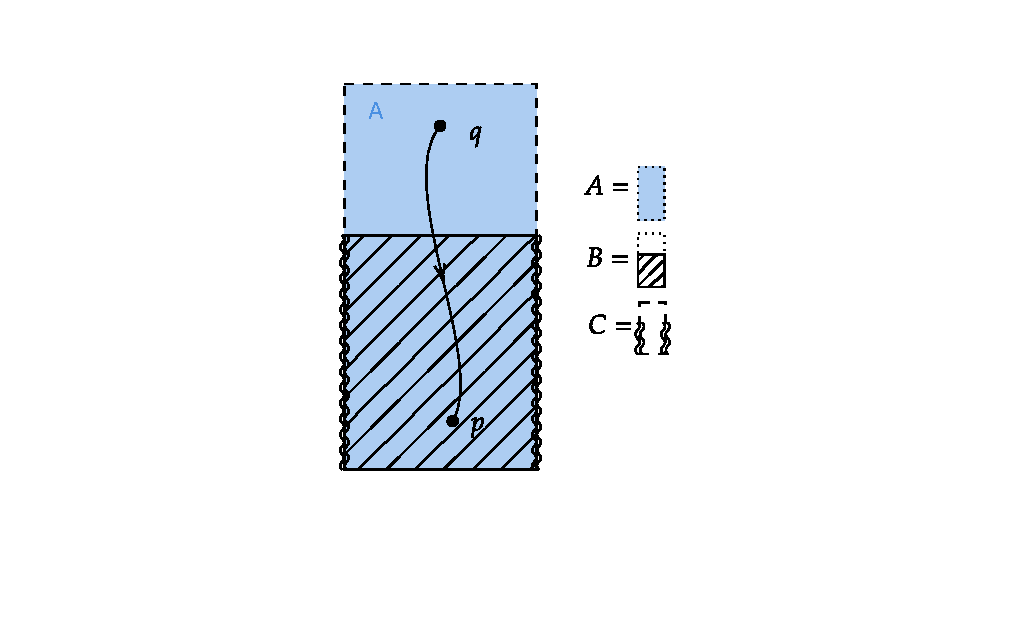
\includegraphics{Text/Pictures/general Proof idea.pdf}
	
	From the perspective of K-theory a regular index pair for a critical point is the same as a sphere with the dimension beeing the index of said critical point. To see this just use a small index pair in a Morse chart (they are all homotopic anyway), collaps the stable part and quotiend by the exit set. By doing this we get the communative diagramm:
	\begin{center}
		% https://tikzcd.yichuanshen.de/#N4Igdg9gJgpgziAXAbVABwnAlgFyxMJZABgBpiBdUkANwEMAbAVxiRAGkA9YAawFoAjAF8AFACFSAYQCUIIaXSZc+QigHkqtRizZdeogIKkxs+Yux4CRMgM31mrRB279hIgMovBQ0wpAYLFSJ1W2p7HSc9HlFPXm9fc2UrFDIAJjttR2d9DxcfOU0YKABzeCJQADMAJwgAWyQyEBwIJFSzEGq6pHUmlsQAZnbO+sRG5u6wzLYAHWnYBhw6AH1gHCqsNAYYITk-YdbqcYGhmpGAFkO+wb3Tg96kM6EKISA
		\begin{tikzcd}
			{K^{k-1}(B,C)} \arrow[d] \arrow[r, "\delta_{triple}"] & {K^{k}(A,B)} \arrow[d] \\
			K^{k-1}(S^{k-1}) \arrow[r] \arrow[d]                  & K^{k}(S^{k-1})         \\
			K^{k}(S^{k}) \arrow[ru]                               &                       
		\end{tikzcd}
	\end{center} And as a map between K Groups of spheres, we know that this map corresponds to the question of orientation. Now we have the maps 
	\begin{enumerate}[(a)]
		\item $S^k\to S\vee (B\big/ C)$ induced from an orientation in the unstable manifold arround $p$ together with $-\grad(f)(x_i)$ where $x_i\in W(q\to p)$. 
		\item $S^k \to (A\big/ B)$ induced from an orientation in the unstable manifold arround $q$. 
	\end{enumerate}
	And hence the diagram 
	\begin{center}
		% https://tikzcd.yichuanshen.de/#N4Igdg9gJgpgziAXAbVABwnAlgFyxMJZABgBpiBdUkANwEMAbAVxiRAGkA9YAawF8AFAGUAOiJowYAAgEAhUgGEAlEpB9S6TLnyEUARlJ6qtRizZdegoZx6r1m7HgJEATOWP1mrRB278BAIKksnbGMFAA5vBEoABmAE4QALZIZCA4EEhuJl5sYrAMOHQA+sA48VhoDDB8ahogCclIBumZiC72DYkpiC0ZqXwUfEA
		\begin{tikzcd}
			{K^{k}(S\vee (B,C))} \arrow[rr, "\delta_{triple}"] &                                  & {K^{k}(A,B)} \\
			& K^{k}(S^k) \arrow[ru] \arrow[lu] &             
		\end{tikzcd}
	\end{center}
	The map now factors over The K-Group of a bouquette of $k$-spheres generated over the connecting flow lines. In each such sphere the comparison of orientations happens.
\end{Iprove}

Bevore we start proving this we need the lemma: 

\begin{lemma}\label{lem: The Main Lemma Np is tubular}
	We work in a compact, riemanian, orientable, smooth Manifold $(M,g)$ of dimension $m$ together with a Morse-Smale funktion 
	\begin{align}
		f: M\to \R
	\end{align}
	We assume that $q$ is a critical point of index $k+1$ and $p$ is a critical point of index $k$. we define $f(q)=b$ and $f(p)=a$ and assume that there is no critical point in $f^{-1}(a,b)\subseteq M$. We define the sub and superlevelsets 
	\begin{align}
		M^t:=\{ x\in M | f(x)\leq t \} \quad \text{and}\quad M_t:=\{ x\in M | f(x)\geq t \} \, ,
	\end{align} and the constants 
	\begin{align}
		c \in (a,b) \quad , \quad \epsilon >0 \text{ small } \quad,\quad T>0 \text{ big .}
	\end{align} With this we define the sets: 
	\begin{align}
		N_q  & \coloneq    \{ x\in M_c |f(\phi_{-T}(x))  \leq b+ \epsilon  \}   \, ,  \\
		L_q  & \coloneq    \{ x\in N_q |f(x)             =    c            \}    \, , \\
		N_p  & \coloneq    \{ x\in M^c |f(\phi_T(x))     \geq a-\epsilon   \}    \, , \\
		L_p  & \coloneq    \{ x\in N_p |f( \phi_T(x))    =    a-\epsilon   \} \, ,
	\end{align} and finally: 
	\begin{align}
		C  & \coloneq  N_p \cup N_q  \, ,                     \\
		B  & \coloneq  N_p \cup L_q   \, ,                   \\
		A  & \coloneq  L_p \cup \mathring{(L_q-N_p)} \, .
	\end{align}
	
	We claim that 
	\begin{enumerate}
		\item $(N_q,L_q)$ is a regular index pair for $q$\, . \label{lem: enum: 1}
		\item $(C,B)$ is an index pair for $q$\, .\label{lem: enum: 2}
		\item $(N_p,L_p)$ is a regular index pair for $p$\, .\label{lem: enum: 3}
		\item $(B,A)$ is an index pair for $p$\, .\label{lem: enum: 4}
		\item $N_p$ is a tubular neighbourhood of $W(\to p)\cap M^c$.\label{lem: enum: 5}
	\end{enumerate}
\end{lemma}

\begin{Iprove}
	The statements \ref{lem: enum: 1}-\ref{lem: enum: 4} are easy to proof by the definitions. The regularity can be derived from a general fact for pairs $(X,Y)$ in metric spaces: If $Y$ is closed in $X$ and there is a neighbourhood of $Y$ that is open in $X$ such that $Y$ is a strong deformation retract of $U$. So the only thing left to show is, that $N_p$ is a tubular neighbourhood. In \cite{Salamon1990} in the proof of lemma 3.2 Salamon claims this to be true without a proof (page 119 in the attached source). Similar, in \cite{banyaga2004lectures} Banyaga claims this (also without any argument).
	The Set $N_p$ is sketched in the figure below. 
	The Idea of the proove is as follows: By increasing $T$ (or decreasing $\epsilon$) we can assume $N_p$ to be an arbitrary small neighbourhood of $W(q\to) \cap M^c$. Now using the flow we can push $N_p$ close to $p$ ($\phi_N(N_p)$ for big $N$ ), where we use a tubular nieghbourhood embedding $J$ that overlapps $N_p$. We now need to proof that we can reduce the radii of the fibers in the domain of $J$ in a smooth way such that $J$ actually becomes a embedding onto the $N_p$ (that we pushed close to $p$). For this we will make use of the lambda lemma (in an improved version), which lets us induce a metric from the unstable tangend space of $P$ into the fiberes of $J$ (since they are transversal to the stable set). With this metric we can finally smoothly reduce the radii of our domain of $J$ to end up with the statement, that $\phi_N(N_p)$ is a tubular neighbourhood of a small part of the stable set of $p$ and hence $N_p$ also. The prove is given as an appendix in section \ref{section: Np tubular neighbourhood proove}.
\end{Iprove}
\begin{center}
	
	
	\tikzset{every picture/.style={line width=0.75pt}} %set default line width to 0.75pt        
	\resizebox{\linewidth}{!}{%
		
		
		
		\tikzset{every picture/.style={line width=0.75pt}} %set default line width to 0.75pt      
		
		\tikzset{every picture/.style={line width=0.75pt}} %set default line width to 0.75pt        
		
		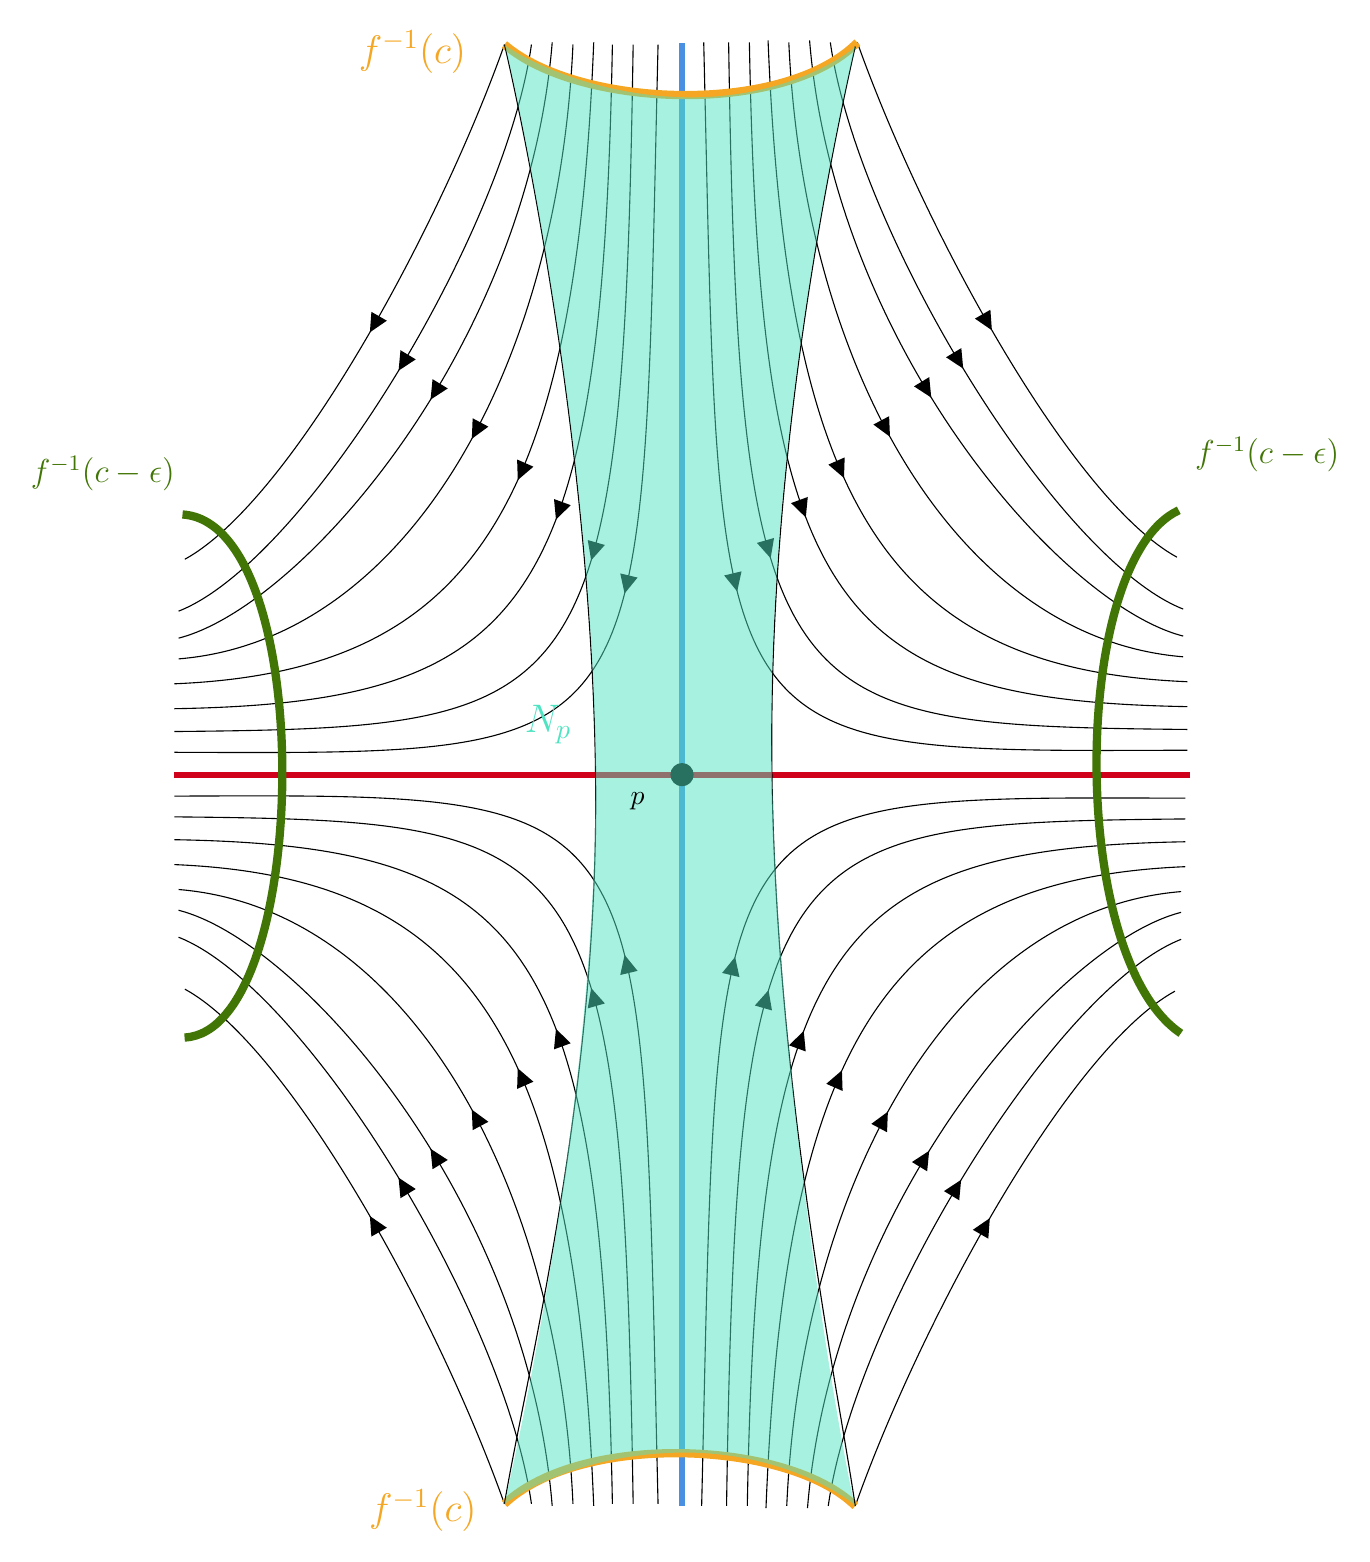
\begin{tikzpicture}[x=0.75pt,y=0.75pt,yscale=-1,xscale=1]
			%uncomment if require: \path (0,843); %set diagram left start at 0, and has height of 843
			
			%Straight Lines [id:da11875089429305197] 
			\draw [color={rgb, 255:red, 74; green, 144; blue, 226 }  ,draw opacity=1 ][line width=2.25]    (329,31.6) -- (329,736.43) ;
			%Straight Lines [id:da5325201497809933] 
			\draw [color={rgb, 255:red, 208; green, 2; blue, 27 }  ,draw opacity=1 ][line width=2.25]    (84.42,384.02) -- (573.58,384.02) ;
			%Shape: Circle [id:dp07579894054308489] 
			\draw  [draw opacity=0][fill={rgb, 255:red, 0; green, 0; blue, 0 }  ,fill opacity=1 ] (323.4,384.02) .. controls (323.4,380.92) and (325.91,378.42) .. (329,378.42) .. controls (332.09,378.42) and (334.6,380.92) .. (334.6,384.02) .. controls (334.6,387.11) and (332.09,389.62) .. (329,389.62) .. controls (325.91,389.62) and (323.4,387.11) .. (323.4,384.02) -- cycle ;
			%Curve Lines [id:da1665503577346341] 
			\draw    (339.45,31.25) .. controls (347.8,378.2) and (336.45,373.05) .. (572.45,372.25) ;
			\draw [shift={(355.57,295.75)}, rotate = 256.55] [fill={rgb, 255:red, 0; green, 0; blue, 0 }  ][line width=0.08]  [draw opacity=0] (8.93,-4.29) -- (0,0) -- (8.93,4.29) -- cycle    ;
			%Curve Lines [id:da7994448259938868] 
			\draw    (351.45,31.25) .. controls (356.45,355.25) and (373.45,360.25) .. (572.45,362.25) ;
			\draw [shift={(371.68,279.76)}, rotate = 253.92] [fill={rgb, 255:red, 0; green, 0; blue, 0 }  ][line width=0.08]  [draw opacity=0] (8.93,-4.29) -- (0,0) -- (8.93,4.29) -- cycle    ;
			%Curve Lines [id:da558792425961241] 
			\draw    (361.45,31.25) .. controls (366.45,302.25) and (401.45,348.25) .. (572.45,351.25) ;
			\draw [shift={(388.63,260.1)}, rotate = 249.87] [fill={rgb, 255:red, 0; green, 0; blue, 0 }  ][line width=0.08]  [draw opacity=0] (8.93,-4.29) -- (0,0) -- (8.93,4.29) -- cycle    ;
			%Curve Lines [id:da5211576581151481] 
			\draw    (370.45,30.25) .. controls (379.45,254.25) and (428.45,333.25) .. (572.45,339.25) ;
			\draw [shift={(407.03,241.09)}, rotate = 246.23] [fill={rgb, 255:red, 0; green, 0; blue, 0 }  ][line width=0.08]  [draw opacity=0] (8.93,-4.29) -- (0,0) -- (8.93,4.29) -- cycle    ;
			%Curve Lines [id:da39021575553782684] 
			\draw    (380.45,31.25) .. controls (387.45,187.25) and (460.45,318.25) .. (570.45,327.25) ;
			\draw [shift={(429.18,221.22)}, rotate = 242] [fill={rgb, 255:red, 0; green, 0; blue, 0 }  ][line width=0.08]  [draw opacity=0] (8.93,-4.29) -- (0,0) -- (8.93,4.29) -- cycle    ;
			%Curve Lines [id:da6126506516051217] 
			\draw    (390.45,30.25) .. controls (402.45,177.25) and (511.45,302.25) .. (570.45,317.25) ;
			\draw [shift={(449.07,202.35)}, rotate = 238.74] [fill={rgb, 255:red, 0; green, 0; blue, 0 }  ][line width=0.08]  [draw opacity=0] (8.93,-4.29) -- (0,0) -- (8.93,4.29) -- cycle    ;
			%Curve Lines [id:da24082042581971141] 
			\draw    (400.45,31.25) .. controls (413.45,123.25) and (509.45,280.25) .. (570.45,304.25) ;
			\draw [shift={(464.47,188.39)}, rotate = 239.04] [fill={rgb, 255:red, 0; green, 0; blue, 0 }  ][line width=0.08]  [draw opacity=0] (8.93,-4.29) -- (0,0) -- (8.93,4.29) -- cycle    ;
			%Curve Lines [id:da5298362087143788] 
			\draw    (413.45,31.25) .. controls (445.45,121.25) and (516.45,251.25) .. (567.45,279.25) ;
			\draw [shift={(478.29,169.92)}, rotate = 240.15] [fill={rgb, 255:red, 0; green, 0; blue, 0 }  ][line width=0.08]  [draw opacity=0] (8.93,-4.29) -- (0,0) -- (8.93,4.29) -- cycle    ;
			
			%Curve Lines [id:da21918221686589523] 
			\draw    (317.45,32.25) .. controls (309.1,379.2) and (320.45,374.05) .. (84.45,373.25) ;
			\draw [shift={(301.33,296.75)}, rotate = 283.45] [fill={rgb, 255:red, 0; green, 0; blue, 0 }  ][line width=0.08]  [draw opacity=0] (8.93,-4.29) -- (0,0) -- (8.93,4.29) -- cycle    ;
			%Curve Lines [id:da34745008178206616] 
			\draw    (305.45,32.25) .. controls (300.45,356.25) and (283.45,361.25) .. (84.45,363.25) ;
			\draw [shift={(285.22,280.76)}, rotate = 286.08] [fill={rgb, 255:red, 0; green, 0; blue, 0 }  ][line width=0.08]  [draw opacity=0] (8.93,-4.29) -- (0,0) -- (8.93,4.29) -- cycle    ;
			%Curve Lines [id:da8640093846313118] 
			\draw    (295.45,32.25) .. controls (290.45,303.25) and (255.45,349.25) .. (84.45,352.25) ;
			\draw [shift={(268.27,261.1)}, rotate = 290.13] [fill={rgb, 255:red, 0; green, 0; blue, 0 }  ][line width=0.08]  [draw opacity=0] (8.93,-4.29) -- (0,0) -- (8.93,4.29) -- cycle    ;
			%Curve Lines [id:da925990106139973] 
			\draw    (286.45,31.25) .. controls (277.45,255.25) and (228.45,334.25) .. (84.45,340.25) ;
			\draw [shift={(249.87,242.09)}, rotate = 293.77] [fill={rgb, 255:red, 0; green, 0; blue, 0 }  ][line width=0.08]  [draw opacity=0] (8.93,-4.29) -- (0,0) -- (8.93,4.29) -- cycle    ;
			%Curve Lines [id:da08743123557319321] 
			\draw    (276.45,32.25) .. controls (269.45,188.25) and (196.45,319.25) .. (86.45,328.25) ;
			\draw [shift={(227.72,222.22)}, rotate = 298] [fill={rgb, 255:red, 0; green, 0; blue, 0 }  ][line width=0.08]  [draw opacity=0] (8.93,-4.29) -- (0,0) -- (8.93,4.29) -- cycle    ;
			%Curve Lines [id:da08430775562121551] 
			\draw    (266.45,31.25) .. controls (254.45,178.25) and (145.45,303.25) .. (86.45,318.25) ;
			\draw [shift={(207.83,203.35)}, rotate = 301.26] [fill={rgb, 255:red, 0; green, 0; blue, 0 }  ][line width=0.08]  [draw opacity=0] (8.93,-4.29) -- (0,0) -- (8.93,4.29) -- cycle    ;
			%Curve Lines [id:da38820398572752524] 
			\draw    (256.45,32.25) .. controls (243.45,124.25) and (147.45,281.25) .. (86.45,305.25) ;
			\draw [shift={(192.43,189.39)}, rotate = 300.96] [fill={rgb, 255:red, 0; green, 0; blue, 0 }  ][line width=0.08]  [draw opacity=0] (8.93,-4.29) -- (0,0) -- (8.93,4.29) -- cycle    ;
			%Curve Lines [id:da5677669307058717] 
			\draw    (243.45,32.25) .. controls (211.45,122.25) and (140.45,252.25) .. (89.45,280.25) ;
			\draw [shift={(178.61,170.92)}, rotate = 299.85] [fill={rgb, 255:red, 0; green, 0; blue, 0 }  ][line width=0.08]  [draw opacity=0] (8.93,-4.29) -- (0,0) -- (8.93,4.29) -- cycle    ;
			
			%Curve Lines [id:da5375642083324416] 
			\draw    (338.45,736.36) .. controls (346.8,389.41) and (335.45,394.56) .. (571.45,395.36) ;
			\draw [shift={(354.57,471.87)}, rotate = 103.45] [fill={rgb, 255:red, 0; green, 0; blue, 0 }  ][line width=0.08]  [draw opacity=0] (8.93,-4.29) -- (0,0) -- (8.93,4.29) -- cycle    ;
			%Curve Lines [id:da5126738644229648] 
			\draw    (350.45,736.36) .. controls (355.45,412.36) and (372.45,407.36) .. (571.45,405.36) ;
			\draw [shift={(370.68,487.86)}, rotate = 106.08] [fill={rgb, 255:red, 0; green, 0; blue, 0 }  ][line width=0.08]  [draw opacity=0] (8.93,-4.29) -- (0,0) -- (8.93,4.29) -- cycle    ;
			%Curve Lines [id:da5839119584885231] 
			\draw    (360.45,736.36) .. controls (365.45,465.36) and (400.45,419.36) .. (571.45,416.36) ;
			\draw [shift={(387.63,507.52)}, rotate = 110.13] [fill={rgb, 255:red, 0; green, 0; blue, 0 }  ][line width=0.08]  [draw opacity=0] (8.93,-4.29) -- (0,0) -- (8.93,4.29) -- cycle    ;
			%Curve Lines [id:da975815253328843] 
			\draw    (369.45,737.36) .. controls (378.45,513.36) and (427.45,434.36) .. (571.45,428.36) ;
			\draw [shift={(406.03,526.52)}, rotate = 113.77] [fill={rgb, 255:red, 0; green, 0; blue, 0 }  ][line width=0.08]  [draw opacity=0] (8.93,-4.29) -- (0,0) -- (8.93,4.29) -- cycle    ;
			%Curve Lines [id:da9314613290760876] 
			\draw    (379.45,736.36) .. controls (386.45,580.36) and (459.45,449.36) .. (569.45,440.36) ;
			\draw [shift={(428.18,546.4)}, rotate = 118] [fill={rgb, 255:red, 0; green, 0; blue, 0 }  ][line width=0.08]  [draw opacity=0] (8.93,-4.29) -- (0,0) -- (8.93,4.29) -- cycle    ;
			%Curve Lines [id:da09174306781681929] 
			\draw    (389.45,737.36) .. controls (401.45,590.36) and (510.45,465.36) .. (569.45,450.36) ;
			\draw [shift={(448.07,565.26)}, rotate = 121.26] [fill={rgb, 255:red, 0; green, 0; blue, 0 }  ][line width=0.08]  [draw opacity=0] (8.93,-4.29) -- (0,0) -- (8.93,4.29) -- cycle    ;
			%Curve Lines [id:da21494064860512774] 
			\draw    (399.45,736.36) .. controls (412.45,644.36) and (508.45,487.36) .. (569.45,463.36) ;
			\draw [shift={(463.47,579.22)}, rotate = 120.96] [fill={rgb, 255:red, 0; green, 0; blue, 0 }  ][line width=0.08]  [draw opacity=0] (8.93,-4.29) -- (0,0) -- (8.93,4.29) -- cycle    ;
			%Curve Lines [id:da506519829239\end{proo7652] 
				\draw    (412.45,736.36) .. controls (444.45,646.36) and (515.45,516.36) .. (566.45,488.36) ;
				\draw [shift={(477.29,597.7)}, rotate = 119.85] [fill={rgb, 255:red, 0; green, 0; blue, 0 }  ][line width=0.08]  [draw opacity=0] (8.93,-4.29) -- (0,0) -- (8.93,4.29) -- cycle    ;
				
				%Curve Lines [id:da3880154567702636] 
				\draw    (317.45,735.36) .. controls (309.1,388.41) and (320.45,393.56) .. (84.45,394.36) ;
				\draw [shift={(301.33,470.87)}, rotate = 76.55] [fill={rgb, 255:red, 0; green, 0; blue, 0 }  ][line width=0.08]  [draw opacity=0] (8.93,-4.29) -- (0,0) -- (8.93,4.29) -- cycle    ;
				%Curve Lines [id:da9327211409936709] 
				\draw    (305.45,735.36) .. controls (300.45,411.36) and (283.45,406.36) .. (84.45,404.36) ;
				\draw [shift={(285.22,486.86)}, rotate = 73.92] [fill={rgb, 255:red, 0; green, 0; blue, 0 }  ][line width=0.08]  [draw opacity=0] (8.93,-4.29) -- (0,0) -- (8.93,4.29) -- cycle    ;
				%Curve Lines [id:da09647590503157577] 
				\draw    (295.45,735.36) .. controls (290.45,464.36) and (255.45,418.36) .. (84.45,415.36) ;
				\draw [shift={(268.27,506.52)}, rotate = 69.87] [fill={rgb, 255:red, 0; green, 0; blue, 0 }  ][line width=0.08]  [draw opacity=0] (8.93,-4.29) -- (0,0) -- (8.93,4.29) -- cycle    ;
				%Curve Lines [id:da15668737739736305] 
				\draw    (286.45,736.36) .. controls (277.45,512.36) and (228.45,433.36) .. (84.45,427.36) ;
				\draw [shift={(249.87,525.52)}, rotate = 66.23] [fill={rgb, 255:red, 0; green, 0; blue, 0 }  ][line width=0.08]  [draw opacity=0] (8.93,-4.29) -- (0,0) -- (8.93,4.29) -- cycle    ;
				%Curve Lines [id:da5883237308999977] 
				\draw    (276.45,735.36) .. controls (269.45,579.36) and (196.45,448.36) .. (86.45,439.36) ;
				\draw [shift={(227.72,545.4)}, rotate = 62] [fill={rgb, 255:red, 0; green, 0; blue, 0 }  ][line width=0.08]  [draw opacity=0] (8.93,-4.29) -- (0,0) -- (8.93,4.29) -- cycle    ;
				%Curve Lines [id:da9204033290837756] 
				\draw    (266.45,736.36) .. controls (254.45,589.36) and (145.45,464.36) .. (86.45,449.36) ;
				\draw [shift={(207.83,564.26)}, rotate = 58.74] [fill={rgb, 255:red, 0; green, 0; blue, 0 }  ][line width=0.08]  [draw opacity=0] (8.93,-4.29) -- (0,0) -- (8.93,4.29) -- cycle    ;
				%Curve Lines [id:da49739155745577546] 
				\draw    (256.45,735.36) .. controls (243.45,643.36) and (147.45,486.36) .. (86.45,462.36) ;
				\draw [shift={(192.43,578.22)}, rotate = 59.04] [fill={rgb, 255:red, 0; green, 0; blue, 0 }  ][line width=0.08]  [draw opacity=0] (8.93,-4.29) -- (0,0) -- (8.93,4.29) -- cycle    ;
				%Curve Lines [id:da32213499249738287] 
				\draw    (243.45,735.36) .. controls (211.45,645.36) and (140.45,515.36) .. (89.45,487.36) ;
				\draw [shift={(178.61,596.7)}, rotate = 60.15] [fill={rgb, 255:red, 0; green, 0; blue, 0 }  ][line width=0.08]  [draw opacity=0] (8.93,-4.29) -- (0,0) -- (8.93,4.29) -- cycle    ;
				
				
				%Curve Lines [id:da05541171078629925] 
				\draw [color={rgb, 255:red, 245; green, 166; blue, 35 }  ,draw opacity=1 ][line width=3]    (243.45,32.25) .. controls (279.42,63.08) and (378.33,66.67) .. (413.45,31.25) ;
				%Curve Lines [id:da4989004892868002] 
				\draw [color={rgb, 255:red, 245; green, 166; blue, 35 }  ,draw opacity=1 ][line width=3]    (243.45,735.36) .. controls (280.33,700.67) and (380.33,704.67) .. (412.45,736.36) ;
				%Curve Lines [id:da44411839842500755] 
				\draw [color={rgb, 255:red, 65; green, 117; blue, 5 }  ,draw opacity=1 ][line width=3]    (88.33,258.67) .. controls (154.22,262.97) and (150.33,507.67) .. (89.33,510.67) ;
				%Curve Lines [id:da05367202270104565] 
				\draw [color={rgb, 255:red, 65; green, 117; blue, 5 }  ,draw opacity=1 ][line width=3]    (568.33,256.67) .. controls (516.33,280.67) and (514.33,471.67) .. (569.33,508.67) ;
				%Curve Lines [id:da7969530986481941] 
				\draw    (243.45,32.25) .. controls (254.33,78.67) and (285.1,230.49) .. (287.33,382.67) .. controls (289.57,534.85) and (253.34,675.31) .. (243.45,735.36) ;
				%Curve Lines [id:da5283140439270424] 
				\draw    (412.45,33.25) .. controls (400.33,86.67) and (370.1,232.49) .. (372.33,384.67) .. controls (374.57,536.85) and (404.33,680.67) .. (412.45,736.36) ;
				
				%Shape: Polygon Curved [id:ds3817941045439226] 
				\draw  [draw opacity=0][fill={rgb, 255:red, 80; green, 227; blue, 194 }  ,fill opacity=0.5 ] (243.45,735.36) .. controls (243.39,735.01) and (288.33,547.67) .. (287.33,382.67) .. controls (286.33,217.67) and (244.39,31.96) .. (243.45,32.25) .. controls (242.51,32.54) and (278.33,56.67) .. (330.33,57.67) .. controls (382.33,58.67) and (412.39,33.99) .. (412.45,33.25) .. controls (412.51,32.51) and (368.33,212.67) .. (372.33,384.67) .. controls (376.33,556.67) and (411.01,736.21) .. (412.45,736.36) .. controls (413.89,736.52) and (381.33,709.67) .. (327.33,710.67) .. controls (273.33,711.67) and (243.51,735.72) .. (243.45,735.36) -- cycle ;
				
				% Text Node
				\draw (303,391.4) node [anchor=north west][inner sep=0.75pt]    {$p$};
				% Text Node
				\draw (172,24.4) node [anchor=north west][inner sep=0.75pt]  [font=\Large,color={rgb, 255:red, 245; green, 166; blue, 35 }  ,opacity=1 ]  {$f^{-1}( c)$};
				% Text Node
				\draw (177,727.07) node [anchor=north west][inner sep=0.75pt]  [font=\Large,color={rgb, 255:red, 245; green, 166; blue, 35 }  ,opacity=1 ]  {$f^{-1}( c)$};
				% Text Node
				\draw (14,229.4) node [anchor=north west][inner sep=0.75pt]  [font=\large,color={rgb, 255:red, 65; green, 117; blue, 5 }  ,opacity=1 ]  {$f^{-1}( c-\epsilon )$};
				% Text Node
				\draw (575,220.4) node [anchor=north west][inner sep=0.75pt]  [font=\large,color={rgb, 255:red, 65; green, 117; blue, 5 }  ,opacity=1 ]  {$f^{-1}( c-\epsilon )$};
				% Text Node
				\draw (252,349.4) node [anchor=north west][inner sep=0.75pt]  [font=\Large,color={rgb, 255:red, 80; green, 227; blue, 194 }  ,opacity=1 ]  {$N_{p}$};
				
				
			\end{tikzpicture}
			
			
		}
	\end{center}
	
	The same arguments work to show that $N_q$ is a tubular neighbourhood of $W(q\to)\cap M_c$, by replacing $f$ with $-f$. Furthermore, we can assume, that the $V_j$ from below are fibers in the normal neighbourhood. This can be realized, since $V_j$ intersect transversal and by trivialization we have a global fram of the bundel and hence can smoothly rescale the embedding along the frame to get that $V_j$ is the image of the fibre above $x_j$. 
	
	
	
	
	
	
	
	
	
	
	
	\begin{proof}[Proof of Theorem \ref{thm: commuting connecting homomorphism}]
		We first notice, that we have the map of triples given by the inclusion:
		\begin{align*}
			\left( ~W(q\to)\cap N_q ~,~S(q\to)~,~S(q\to ) \setminus \bigcup\limits_jV_j ~\right) \to (C,B,A)
		\end{align*} and hence by naturalitiy we have the diagram, where the top square commutes:
		\begin{fdiagram}
			% https://tikzcd.yichuanshen.de/#N4Igdg9gJgpgziAXAbVABwnAlgFyxMJZABgBpiBdUkANwEMAbAVxiRAGkA9YAWgB0+DOgFsARlDoB9NAF8BDGADMcyAAQAhUgEFVAgE5YA5gAscFEDNLpMufIRQBGclVqMWbLr3kjxUgI5ygkoqAMKkGrp8BiZmFlYgGNh4BERkDi70zKyIHNz8gj4S0oEKymoAygAUfgI4EACUpFU1fHX1AnAwOMJYYExwkaJGAMZMaPJYPThwkgBWkb14lQBqc-WR0abmltZJdkRO6dSZ7jme+UJiRQHywcgA6tW1DQLDdGiqAHLSTU+tDRsjFs4rtbCkUGQAEwZNzZXJeApXKSyW5lVSrWakARoOh6PCMdFzQExbYuGBQQzwIigRR6CDCJBkEB1JBOEBCUQwBgABRsyXs7OCIGOsLYAlgDBwUmAOAMaAUMk4DhBIFp9MZ1BZiEhIqybCwkmAmi0ioAVCq1QzEGytQBmXWnEAG4BhdRmi10q065kQJD21x6nLirlSw2yrDymCKyEe9XazW+xAAFgdcINs045uoHK5vL24JAmxwwpAcGMWGUSEhO1VnqQKZ9ftTYr4EqlnFmYblCpLOZ5fP2OSLsatDa13pOcOGc0zvbonP7+YFw5kFBkQA
			\begin{tikzcd}
				{K^{-\lambda_p}\left[ B,A \right]} \arrow[r, "\delta_{triple}^1"] \arrow[d, "{i_{B,A}^*}"]                                                            & {K^{-\lambda_q}\left[C, B \right]} \arrow[d, "{i_{C,B}^*}"] \\
				{K^{-\lambda_p}\left[ S(q\to),S(q\to)\setminus \bigcup\limits_j \inti(V_j) \right]} \arrow[r, "\delta_{triple}^2"] \arrow[d, "i_j^*"', shift right=2] & {K^{-\lambda_q}\left[W(q\to)\cap N_p,S(q\to) \right]}       \\
				{K^{-\lambda_p}\left[ V_j,\partial V_j \right]} \arrow[ru, "\delta^j_{triple}"'] \arrow[u, "c_j^*"']                                                  &                                                            
			\end{tikzcd} 
		\end{fdiagram}
		\noindent	Furthermore, in this diagram the tuple $\left(K^{-\lambda_p}\left[ S(q\to),S(q\to)\setminus \bigcup\limits_j \inti(V_j) \right],\left(c_j^*\right)_j\right)$ is a coproduct, and we define  $\delta^j_{triple}\coloneq \delta^2_{triple}\circ c_j^*$. Then we have that 
		\begin{equation*}
			\delta^2_ {triple}=\sum_j\delta^j_{triple}\circ i_j^*
		\end{equation*}
		Since $i_{C,B}^*$ is an isomorphism (since $W(q\to \cap N_p$ is a deformation retract of $C$ and the collaps collapses $B$ to $S(q\to)$), we have that 
		\begin{equation} \label{eq: Delta in terms of delta j}
			\Delta(\alpha_q)=\delta^1_{triple}(\alpha_q)=i^*_{C,B}\circ \sum_j\delta^j_{triple}\circ i_j^* \circ i^*_{B,A}(\alpha_q)
		\end{equation}
		
		The map $\delta^2_{triple}$ is defined as the composition:
		\begin{fdiagram} \label{diag: Definitino of delta j}
			\begin{adjustbox}{max width=\textwidth}
				% https://tikzcd.yichuanshen.de/#N4Igdg9gJgpgziAXAbVABwnAlgFyxMJZABgBoBGAXVJADcBDAGwFcYkQBpAPWAFoAdfo3oBbAEZR6AfTQBfQYxgAzHMgAEAZQAUAR0E4IASlLa9-A4cFwYOEVjDM4awWKwBzAMbM0CrHZxwUgBWzvz2eFoAasGGoQBO7gAWOJQgsqTomLj4hChkAEzUdEys7Nx8CqIS0nIKyqqauvpG8UkpaRkgGNh4BETkpIU0DCxsiJw8AkJVkjIA1OTyQvXIGlLkgrQwMI1mFq1uyanpmT05RPmDRSOl4+VTwuKzaAtLiirIAOpN5kaCHvQ0GoAHIyf7eNQAYXWdRUWl2zUs-AShxwxm+ez+-ABQNBQMEKKOHVO2T6KAAzFdhiUxhMKtMnjVXrDVBjEf9ASCwdiIdCNss4QjfkjCWiCW1jp1uqTcshKVRqaMypNKoypDo3is2cKObiZCYfvtxajJSTerKyMRrjTlfTHtUZJqPmpokFSII0PQ4ngmC7ggcibIijAoG54ERQEo4hAREgyCADEgBsUleMsOsuAAqYkgKMxpM0ROIS4p24gRJZ9Y5vOx4uFiBISml2mJKT5LPV6O1ptFgAsirL6fb2ZOua7SH7CYbiAArAPaS4bPR-lg4h5QjgYAAPHDAHAJWiyKTAPmmRGyTv5xDxotz5vsQSwRg4ehcfLH-dYNCKC+jmtIAA2es43ndgPGCDsg1kIA
				\begin{tikzcd}
					{K^{-\lambda_p}\left[ V_j,\partial V_j \right]} \arrow[d, "c_j^*"]                                                                      &                                                                    &                                                                                                                 &                                                                                                                              \\
					{K^{-\lambda_p}\left[ S(q\to),S(q\to)\setminus \bigcup\limits_j \inti(V_j) \right]} \arrow[d, "i_1^*"] \arrow[rrr, "\delta^2_{triple}"] &                                                                    &                                                                                                                 & {K^{-\lambda_q}\left[W(q\to)\cap N_p,S(q\to) \right]}                                                                        \\
					{K^{-\lambda_p}\left[ S(q\to) \right]} \arrow[r, "h^*_1"]                                                                               & {K^{-\lambda_p+1}\left[S_1\vee S(q\to) \right]} \arrow[r, "h_2^*"] & {K^{-\lambda_p+1}\left[W(q\to)\cap N_p\cup C_1\left( S(q\to)\right),W(q\to)\cap N_p \right]} \arrow[r, "i_2^*"] & {K^{-\lambda_p+1}\left[W(q\to)\cap N_p\cup C_1\left( S(q\to)\right)\right]} \arrow[u, "\beta\circ \text{triv}_{C_1S(q\to)}"]
				\end{tikzcd}
			\end{adjustbox}
		\end{fdiagram}
		
		The downwards maps in the theorem are the induction of the canonical generators. This is done by the following assignement
		
		
		
		Now the composition \begin{equation*}
			h_1*i_1*\circ c_j*: K^{-\lambda_p}\left[ V_j,\partial V_j \right] \to K^{-\lambda_p+1}\left[S_1\vee S(q\to) \right]
		\end{equation*} can be simplified by the map
		\begin{equation*}
			l^*:	K^{-\lambda_p}\left[ V_j,\partial V_j \right]=K^{-\lambda_p+1}\left[S_1\vee\left( V_j,\partial V_j\right) \right] \to K^{-\lambda_p+1}\left[S_1\vee S(q\to) \right]
		\end{equation*} where l is the collapsing map.
		\begin{align*}
			l:S_1\vee S(q\to)  \to S_1\vee\left( V_j,\partial V_j\right)\\
			(t,x)\mapsto (t,\overline{x})
		\end{align*} So now we are in the following situation: 
		\begin{fdiagram}
			\begin{adjustbox}{max width=\textwidth}
				% % https://tikzcd.yichuanshen.de/#N4Igdg9gJgpgziAXAbVABwnAlgFyxMJZABgBpiBdUkANwEMAbAVxiRAGkA9YAWgB0+DOgFsARlDoB9NAF8BDGADMcyAGqSAVqQFo6AJzyMABOo1GBerAHMAFjgogZpdJlz5CKAEzkqtRizYuXnkRcSkARzlBJRUAdQAKcPM+HAgjAEoBAGM6NCMAOWlSAGVEgVTMvktbe0dnEAxsPAIib09femZWRA5ufkFQiWkeAEYohWVkAWE6HBtRUWBimW4QsSG0AGox5Oq7BycXJvciMnbqToCeoP6hdak0UfGYqb4ZuYWlleA1sOltmS7az7OpHNwtFAjUgjDr+bq9YIDe7-MbyF5GYqSEYCGgwGAYsopCCVPa1GS+GBQKzwIigRR6CDCJAAZmoqSQZD8XTYimknAAVKCQPTGUhvCB2YgoVyrsLJOEBUKRUzEJzJdLLvCBLAGDg6JwNJJgDhLGgFDIlQyVayJRAxYdhVaWWy7YgACwXOFsOCKh3KpAe21iz3cnp6X31f2ql0BkOyhhYiN0p3umNSuPwhOeRwUGRAA
				\begin{tikzcd}
					{K^{-\lambda_p}\left[V_j,\partial V_j \right]} \arrow[rr, "\delta^j_{triple}"] \arrow[rd, "l_1^*"]        &                                                                                     & {K^{-\lambda_q}\left[W(q \to )\cap N_p,S(q\to)\right]}                       \\
					& {K^{-\lambda_p+1}\left[ S_1\vee S(q\to)\right]} \arrow[rd, "r^*"] \arrow[ru, "l_2"] &                                                                              \\
					{K^{-\lambda_p-1}\left[\mathbb{S}^{\lambda_p+1} \right]} \arrow[uu, "f_p^*"] \arrow[rr] \arrow[ru, "s^*"] &                                                                                     & {K^{-\lambda_p-1}\left[\mathbb{S}^{\lambda_p+1} \right]} \arrow[uu, "f_q^*"]
				\end{tikzcd}
			\end{adjustbox}
		\end{fdiagram}
		The maps in the diagramm are given as follows:
		\begin{itemize}
			\item The map $f_p$ induces $\alpha_p$. Remember, that $\alpha_p$ comes from the canonical generator $\alpha_p'$ of the index pair $[B,A]$ and $\alpha_p'$ is defined as
			\begin{align*}
				(\phi\circ{ \tilde{\psi}}^{-1})^*(\beta)~\text{where }& \phi \text{ is the homotopie equivalence of index pairs}\\
				& \tilde{\psi} \text{ is a Morse chart adapted to the basis of } T^u_pM,\\
				\text{and }& \beta \text{ is the bott generator of the sphere } [D^u_\epsilon\times D^s_\epsilon\Big/ \partial D^u_\epsilon\times D^s_\epsilon
				\,				.
			\end{align*} Instead of using $\phi$ we can rescale $\tilde{\psi}$ to be a mapping to $[B,A]$ instead of first mapping to the prototype index pair $[D^u_\epsilon\times D^s_\epsilon,\partial D^u_\epsilon\times D^s_\epsilon]$. 
			We call this rescaled Morse chart $\psi$. 
			Then $\psi^{-1}(\beta)= (\phi\circ{ \tilde{\psi}}^{-1})^*(\beta)$ since the map $\tilde{\psi}\circ \phi^{-1}\circ \psi^{-1}$ has the local and hence global degree one. (this can be checkt by differentiataion at the origin). Hence $\alpha_p'=(\psi^{-1})^*(\beta)$. The inclusion 
			\begin{equation*}
				i_p: (V_j,\partial V_j)\to (B,A)
			\end{equation*} induces an isomorphism in the K-groups since $N_p$ is a tubular neighbourhood of the contractible $W(\to p)\cap M^c$ and the contraction to the fiber $V_j$ contracts $L_p$ to $\partial V_j$ (the contraction is well defined on the quotients, and for K-THeory, we only care for the qutoient spaces). Now $\alpha_p''=i_p^*(\alpha_p')$. Define the two funktions
			\begin{align*}
				J: \mathcal{N}^{W(q\to)} W(\to p)\cap M^c \to N_p \text{ the normal neighbourhood embedding,  }\\
				\nu: \mathcal{N}^{W(q\to)} W(\to p)\cap M^c \to  W(\to p)  \times T^u_pM \text{ The trivialization of the normal bundle.}  
			\end{align*}
			Define $\mathfrak{b}^p$ to be an ordered basis of $T^u_pM $ that is compatible to the orientation of said tanged space. Then assume that $J$ is defined, such that 
			\begin{align*}
				\left(B_{\mathfrak{b}^p}^{-1}\circ \nu_{x_j}\circ J^{-1}\right)^*(\beta)=\alpha_p'' \,.
			\end{align*} If this is not the case just compose $J$ with a basechage of degree one. Now $\alpha_p''$ generates $K^{-\lambda_p}(V_j,\partial V_j)$. The latter is isomoprhic to $K^{-\lambda_p+1}(I\times V_j,\partial(I\times  V_j))$ by definition. Now we denote the suspensision is the wedge produkt with a sphere. Hence for $K^{-\lambda_p+1}(I\times V_j,\partial(I\times  V_j))$ we can induce the generator by the function
			\begin{align*}
				f_p: I\times V_j \Big/ \partial(I\times V_j) &\to S \wedge S^{\lambda_p}\simeq  S^{\lambda_p+1}\\
				(t,x)&\mapsto \Omega\left(t,	\Gamma\circ \left(B_{\mathfrak{b}^p}^{-1}\circ \nu_{x_j}\circ J^{-1}\right)(x)\right) \, .
			\end{align*}
			$\Gamma$ maps the disk modulo its boundary to a sphere and $\Omega$ maps the suspension of the sphere to the sphere one dimension higher These Maps are given in definitino \ref{cor: suspension of a sphere is a sphere} and \ref{def: Disk modulo boundary to sphere}. We abuse the notation a bit and identify the map $\left(B_{\mathfrak{b}^p}^{-1}\circ \nu_{x_j}\circ J^{-1}\right)$ with the one defined by quotiening out the boundary. We will leave out the quotiening in the notatino from now on to make the prove easyer to read. The invested reader should check, if the quotiend maps are always well defined! Now finally we have a little definition issue: In the diagramm we have that 
			\begin{equation*}
				f_p^*: K^{\lambda_p-1}[\mathbb{S}^{\lambda_p+1}]\to K^{-\lambda_p}[V_j,\partial V_j]\, ,
			\end{equation*}whilst at the moment, $f_p$ maps to $K^{-\lambda_p-1}(I\times V_j,\partial(I\times  V_j))$. Hence we need to compose this $f_p^*$ with the isomorphism that comes from the suspension axiom: 
			\begin{equation*}
				K^{-\lambda_p}( X)\cong K^{-\lambda_p+1}(SX)\,.
			\end{equation*}And then add the bott isomorphism to rais th eindex by two. By abuse of notation we dont write that idetification and rather think of the top left corner as $K^{-\lambda_p+1}(I\times V_j,\partial(I\times  V_j))$.
			\item Again, we want $f_q$ to be the map that induces the generator of $K^{-\lambda_q}[W(q\to)\cap N_q,S(q\to)]$ which comes from the canonical generator of $[C,B]$ together with the inclusion. Again instead of first introducing the generator on the prototype index pair, we can use ${E^u_q}^{-1}$ instead of the Morse chart. Again we can argue here, that the local degree of changing between the two is one, since ${E^u_q}^{-1}$ is a refined morse chart which can be choosen to be adapted to the ordered basis $\mathfrak{b}^q$ of $T^u_qM$.´ Hence we can define $f_q$ to be the quotient map:
			\begin{align*}
				W(q\to)\cap N_q\Big/ S(q\to)& \to S^{\lambda_p+1}\\
				x& \mapsto \Gamma\circ  B_{\mathfrak{b}^q}^{-1}\circ {E^u_q}^{-1}(x)\,.
			\end{align*} Here $\Gamma$ maps the disk modulo its boundary to the sphere. 
			Hence $f_q=\left(B_{\mathfrak{b}^q}^{-1} \circ {E^u_q}^{-1}\right)^*:K^{}$
			\item The map $l_1$ is the collapsing map 
			\begin{equation*}
				S_1\wedge S(q\to)\to S_1 \wedge (V_j\big/ \partial V_j)
			\end{equation*}
			\item The map $l_2$ is not topologically induced. 
			\item The map $s$ is given by $f_p\circ l_1$. Again we abuse the notation and leave out the suspension isomorphism when 
			\begin{equation*}
				s^*: K^{-\lambda_p+1}[S_1\wedge S(q\to)]\to K^{-\lambda_p-1}[\mathbb{S}^{\lambda_p+1}]\,.
			\end{equation*}
			\item To find the map $r$ that fits the diagram (to make it commute) is the next goal. First we need to dig into $l_2$: From diagram \ref{diag: Definitino of delta j} we know that $l_2=\Sigma \circ \text{triv}_{C_1S(q\to)}\circ i_2^*\circ h_2^*$, Where $\Sigma$ denotes the suspension isomorphism. Hence, if the function $r^*$ makes the diagram commutative we need to ensure, that $f_q^* \circ r^*=l_2$. If we define the function 
			\begin{align*}
				col: W(q\to) \cap N_p \cup C_1  S(q\to) \to S_1 \wedge S(q\to) \,
			\end{align*} 
			to be the collision, of $W(q\to) \cap N_p $ to a point, then
			$i_2^*h_2^*=col^*$. Now while the function  $\text{triv}_{C_1S(q\to)}$ is not topologically induced, its inverse is. Lets call the collaps of $C_1S(q\to)$: 
			\begin{equation*}
				k_1:	\left(W(q\to)\cap N_p \right)\cup C_1S(q\to)\to \left(W(q\to)\cap N_p \middle/ S(q\to) \right) 
			\end{equation*}
			$\pi_1$. Then since $\Sigma$ is a natural transformation we have 
			\begin{equation*}
				f_q^*\circ r^*=l_2\Leftrightarrow k_1^*\circ f_q^*\circ r^*=\Sigma \circ col^*
			\end{equation*}
			Now all maps are topologically induced except $\Sigma$ and the latter is just used to geht the index in the $K$ group right. Hence, if $r$ would be such that
			\begin{equation*}
				r\circ f_q\circ c_1=col\,, 
			\end{equation*}then the requirement on the induced maps would be satisfied. We first however need to formulate a little lemma:
			\begin{lemma}
				Let $S^k\coloneq \{x\in \R^{k+1}|\norm{x}=1\}$, $H_+\coloneq\{x\in S^k|x_0\geq 0\}$ denote the upper hemissphere, $H_-$ the lower hemissphere,  $\pi:S^k \to D^k$ with $\pi(x_0,\dots,x_{k})=(x_1,\dots x_k)$ be the projection and $\Lambda$ be the homeopmorphism from $D^k\big/\partial D^k \to S^k$. Let furthermore $c_{Eq}:S^k\to \overline{H_+}\vee \overline{H_-}$ be the collaps of the equator, where $\overline{H_+}$ denotes the upper hemisphere modulo the equator and $\overline{H_-}$ is defined analog. Let finally $c_2: \overline{H_+}\vee \overline{H_-} \to \overline{H_+}$ be the collaps of the second summand and analogusly $c_1:  \overline{H_+}\vee \overline{H_-} \to \overline{H_-}$. Then we have that $\Lambda\circ \pi\circ c_2\circ c_{Eq}\simeq -\Lambda\circ \pi\circ c_1\circ c_{Eq}$, where de minus denotes any smooth homotopie equivalence of negative degree. 
			\end{lemma}
			\begin{proof}
				This lemma is the concrete version of a standart lemma that is often formulated along the lines: Let $q:S^k\to S^k\vee S^k$ be the collaps of the equator and $p_i$ be the projection to the $i$-th summand, then $p_1\circ q=-p_2\circ q$.  
			\end{proof}
			Now we need to transport our situation to fit the lemma. For this we will use the maps defined in the lemma above, and need a bunch of maps again: 
			\begin{itemize}
				\item Firts, the map $\rho$ is given by 
				\begin{align*}
					\rho: W(q\to)\setminus \{q\}&\to W(q\to)\cap f^{-1}(c)\setminus W(q\to)\setminus \{q\}\\
					x\mapsto \phi_{\tau(x)}(x)\,,
				\end{align*} and 
				\begin{align*}
					\tau: W(q\to)\setminus \{q\} &\to \R\\
					x                  &\mapsto \tau(x) \text{ such that }f\circ \phi_{\tau(x)}(x) =c \, .
				\end{align*}
				\item $\Phi:S^{\lambda_q}\to W(q\to) \cap N_p\cup C_1S(q\to)$ is defined with a case distingtion. We define 
				\begin{align*}
					\restr{\Phi}{{H}_+}(x)&=E^u_q\circ B_{\mathfrak{b}^q}^{-1}\circ \pi(x)\\
					\restr{\Phi}{{H}_-}(x)&=(\euler^{\tau(y)},\rho (y))\text{ where }y=E^u_q\circ B_{\mathfrak{b}^q}(\pi_-(x)) \,.
				\end{align*}Notice, how this function is continuous and does not depend on the choice taken in the definition of $\rho'$. 
				\item $\Psi: S^{\lambda_q}\vee S^{\lambda_q}\to \left(W(q\to)\cap N_p \middle/ S(q\to)\right)\vee \mathbb{S}\wedge S(q\to)$ is given by mapping $x\mapsto \overline{\Phi(x)}$. The well definition is easy to see. 
				\item $p_i$ for $i=1,2$ denotes the projection onto the first or second summand in a pointed sum. 
				\item $C_{S(q\to)}:W(q\to)\cap N_q\cup C_1S(q\to) \to \left(W(q\to)\cap N_p \middle/ S(q\to)\right)\vee \mathbb{S}\wedge S(q\to)$ is the collaps of $S(q\to)$. 
				\item $R:\mathbb{S}^{\lambda_q}\to \mathbb{S} \wedge S(q\to)$ is defined to be $col\circ \Phi$ 
			\end{itemize}
			This gives the commutative diagram below, where by the lemma above the upper path is the negative of the lower path.
			\begin{fdiagram}
				\begin{comment}
					\begin{adjustbox}{max width=\textwidth}
						% https://tikzcd.yichuanshen.de/#N4Igdg9gJgpgziAXAbVABwnAlgFyxMJZAJgBpiBdUkANwEMAbAVxiRAB12IaYAnBrGBjAAEgH0A1AF9OPGAAJO3PgKGixAWikgppdJlz5CKMgEYqtRizacAtnRwALAEbPgAZSkA9YJwZ1bZyg6MQBHbV19bDwCIjIAZgt6ZlZEDnZ7J1cPb192f0DgsIi9EAxooyIABnIkq1T0zJc3Tx8-AKCQ8J1S8sNYlFNSc2pk6zT5AHUAClDOHAgASkV2AGM6NHkAOTE0TlWmTYBhMVN3Wfmlnqj+42R40iq6lJt8mAAzHGmZufYFxf2G22uxWtiwUCgDBgAHp5Odfv9OLwsABzRw4RbXMoGGJ3B6UUb1NighzNHKcADuMCgKIU8MumMi2IqA3uw2e43SUM+3wufyWgM2O02dnBkJhcL5iPYyLRGNkMAUdlJ2U8lOptMlCKuUgsGvgRFA714EFsSBqIAWSCGlheaU4ABkOsF9lheKsVmgsCtVm6PasxMQQNR-M4YAwAAo4yppQTYWBY42m83UK2IMi2zmO510V3uz3evP+07BkCh8NRlnGEBx8GsJlJs2IB6WiApzMNAPAACi3RDdDDkejAxrYHj9dKjaQLbTABZCXb0hHHFhEyamza0wBWBvrpAZtMANl3ycQ89bSAA7AvOScPFKliUjXvENeL4gtzeGpwvSX+4PK1uNhawTE8mzfI8v1eX8g3-Cth2rECJ2fU8LTTN8xm-dgI2wUtyyHKtgLHOsdAoKQgA
						\begin{tikzcd}
							&                                                            &                                                                                                                                                                          & \left(W(q\to)\cap N_p \middle/ S(q\to)\right)                                                                                            \\
							&  W(q\to) \cap N_p\cup C_1S(q\to) \arrow[rr, "C_{S(q\to)}"] & \mathbb{S}^{\lambda_q} \arrow[ru]                                                                                                                                        & \left(W(q\to)\cap N_p \middle/ S(q\to)\right)\vee \mathbb{S}\wedge S(q\to) \arrow[u, "\pi_1" description] \arrow[d, "\pi_2" description] \\
							\mathbb{S}^{\lambda_q} \arrow[rr, "c_{Eq}" description] \arrow[ru, "\Phi"] &                                                            & \overline{H_+}\vee \overline{H_-} \arrow[u, "\Lambda\circ \pi \circ c_2" description] \arrow[d, "\Lambda\circ \pi \circ c_1" description] \arrow[ru, "\Psi" description] &  \mathbb{S}\wedge S(q\to)                                                                                                                \\
							&                                                            & \mathbb{S}^{\lambda_q} \arrow[ru]                                                                                                                                        &                                                                                                                                         
						\end{tikzcd}
					\end{adjustbox}
				\end{comment}
			%	
\includegraphics[width=\textwidth]{Text/Pictures/Kommutative Diagram Sphere equator collaps.jpeg.pdf}
			\end{fdiagram}
			Now define $r\coloneq -R$. For example apply $R$ after the reflection $(x_0,\dots x_{\lambda_q})\mapsto (-x_0,\dots,x_{\lambda_q})$. Then by the lemma above and commutativity we have up to homotopy:
			\begin{align*}
				r\circ f_q\circ k_1 
				&=  	-R\circ f_q\circ k_1 \circ \Phi \circ \Phi^{-1}\\
				&=  	-R\circ \Lambda \circ \pi\circ c_2\circ C_{Eq} \circ \Phi^{-1}\\
				&=  	R\circ \underbrace{\Lambda \circ \pi\circ c_1\circ C_{Eq} }_{\simeq \id}\circ\Phi^{-1}\\
				&=		col\, .
			\end{align*}
			
		\end{itemize}  
		With $r$ we finally have all the maps. Now we want to find out what degree the composition
		$s\circ r$ has. For this we calculate the local degree in some point by checking the sign of the determinant of the Jacobean. This strategy works out since we are in the situation of lemma \ref{lem: determined of javobean and collapsing map}.
		Bevor we start differentiating, we expand the map arround $x\in \R^{\lambda_q}$, such that $x'\coloneq E^u_q\circ B_{\mathfrak{b}^q}(x)\in \rho{-1}(x_j)$, meaning that $x'$ is on the flow line towards $x_j$ and assume that $\tau(x')=1$.
		\begin{align*}
			&   \phantom{=}	\pi_+\circ s\circ r\circ \pi_+^{-1}(x_1,\dots .,x_{\lambda_q})\\
			&=	\pi_+\circ s\circ R (- x_0,x_1,\dots .,x_{\lambda_q}) \quad x_0>0\\
			&=	\pi_+\circ s\circ col \circ \restr{\Phi}{H_-} (-x_0,x_1,\dots .,x_{\lambda_q}) \\
			&=	\pi_+\circ f_p\circ l_1 \circ col \left(e^{\tau(x')},\rho(x')\right) \quad \text{ $col$ and $l_q$ are the identity arround $\left(e^{\tau(x')},\rho(x')\right)$ } \\
			&=\pi_+\circ \Omega  \Big(e^{\tau(E^u_q\circ B_{\mathfrak{b}^q}(x))},\Gamma \circ \underbrace{B_{\mathfrak{b}^p}^{-1} \circ \nu_{x_j}\circ J^{-1}\circ \rho \circ E^u_q\circ B_{\mathfrak{b}^q}(x)}_{\coloneq Z(x)}\Big)\\
			&=\sin(\pi e^{\tau(E^u_q\circ B_{\mathfrak{b}^q}(x))}) \cdot
			\begin{pmatrix}
				-\cos\left(\pi \cdot \norm{Z(x)}\right)\\
				\sin\left(\pi \cdot \norm{Z(x)}\right) \cdot \frac{Z(x)}{\norm{Z(x)}})
			\end{pmatrix}
		\end{align*}
		Here $Z$ is a funktion $Z: \inti(I\times D^{\lambda_q})\to \R^{\lambda_q-1}$ and we can calculate its jacobean Notice how $Z(y)=0$ where $y$ is the same as above. We only care for the sign of its jacobean, so we will manipulate the funktion in a way that might change the function, but not the sign of ots Jacobean determinant. 
		Let $Q_y: V\to T_yV$ be the canonical map, that identifies a linear space with the tangendspace of a point from inside said space. Now we calculate:
		
		
		\begin{align*}
			&\phantom{=}Q_0^{-1}\circ \restr{\diff \left(B_{\mathfrak{b}^p}^{-1} \circ \nu_{x_j}\circ J^{-1}\circ \rho \circ E^u_q\circ B_{\mathfrak{b}^q}\right)}{y}\circ Q_y (e_i)\\
			&=Q_0^{-1}\circ  \restr{\diff \left(B_{\mathfrak{b}^p}^{-1} \circ \nu_{x_j}\circ J^{-1}\circ \rho \circ E^u_q\right)}{B_{\mathfrak{b}^q}(y)}\circ Q_{B_{\mathfrak{b}^q}(y)}\circ B_{\mathfrak{b}^q}(e_i) \\
			&= Q_0^{-1}\circ \restr{\diff \left(B_{\mathfrak{b}^p}^{-1} \circ \nu_{x_j}\circ J^{-1}\right)}{x_j}\circ \restr{\diff \left( \rho \circ E^u_q\right)}{B_{\mathfrak{b}^q}(y)}\circ Q_{B_{\mathfrak{b}^q}(y)}\circ B_{\mathfrak{b}^q}(e_i)		
		\end{align*}
		Now the term $\restr{\diff \left( \rho \circ E^u_q\right)}{B_{\mathfrak{b}^q}(y)}\circ Q_{B_{\mathfrak{b}^q}(y)}\circ B_{\mathfrak{b}^q}$ maps $e_1$ to zero. and $(e_2,\dots e_{\lambda_q})$
		induces a basis in $T_{x_j}V_j$ that is compatible with a basis $(\mathfrak{d}_i)_{i=2,\dots \lambda_q}$ that satisfies the following: Adding $-\grad_{x_j}(f)$ as the first basis vector to $(\mathfrak{d}_i)_{i=2,\dots \lambda_q}$ gives a basis of $T_{x_j}W(q\to)$ that is compatible with the basis induced from $\mathfrak{b}^q$ that appears in the counting of flow lines in the Morse boundary operator. This was proven earlyer in lemma \ref{lem: Rho and Tau induces a Morse boundary orientation}.
		Now we can look at the first part: 
		\begin{align*}
			Q_0^{-1}\circ \restr{\diff \left(B_{\mathfrak{b}^p}^{-1} \circ \nu_{x_j}\circ J^{-1}\right)}{x_j}
			&=\Big(\restr{\diff J}{x_j}\circ \restr{\diff \nu_{x_j}^{-1}}{0}\circ \restr{\diff B_{\mathfrak{b}^p}}{0} \circ Q_0 \Big)^{-1}\\
			&=\Big(\underbrace{\restr{\diff J}{x_j}\circ Q_{0}}_{=\id_{T_{x_j}V_j}} \circ \nu_{x_j}^{-1}  \circ B_{\mathfrak{b}^p} \Big)^{-1}\\	
			&=\Big( \nu_{x_j}^{-1}  \circ B_{\mathfrak{b}^p} \Big)^{-1}
		\end{align*}
		Notice how $\nu_{x_j}^{-1}  \circ B_{\mathfrak{b}^p}$ induces a basis on $T_{x_j}V_j$ from a basis in $T^u_pM$. Comparing this basis to the basis  $(\mathfrak{d}_i)_{i=2,\dots \lambda_q}$ is what assigned the sign to the flow line in the Morse boundary operator. By the calculations we know that the Jacobean of the funktion $Z$ 
		\begin{equation*}
			\diff Q_0^{-1}\circ \restr{\diff \left(B_{\mathfrak{b}^p}^{-1} \circ \nu_{x_j}\circ J^{-1}\circ \rho \circ E^u_q\circ B_{\mathfrak{b}^q}\right)}{y}\circ Q_y=
			\begin{pmatrix}
				0&\tilde{Z}
			\end{pmatrix}\,,
		\end{equation*}where $\tilde{Z}$ is a $\lambda_{q-1}$ matrix with the sign of its determinant being given by the sign in the Morse boundary operator $n_{\gamma}$. 
		
		Now we can calculate the differential 
		\begin{align*}
			&   \restr{\diff \Big( \pi_+\circ s\circ r\circ \pi_+^{-1}(x_1,\dots .,x_{\lambda_q})\Big)}{x}\\
			&=  \restr{\diff \left(\sin(\pi e^{\tau(E^u_q\circ B_{\mathfrak{b}^q}(x))}) \cdot
				\begin{pmatrix}
					-\cos\left(\pi \cdot \norm{Z(x)}\right)\\
					\sin\left(\pi \cdot \norm{Z(x)}\right) \cdot \frac{Z(x)}{\norm{Z(x)}})
				\end{pmatrix}\right)}{x}
		\end{align*} To keep it readable we will first calculate
		\begin{equation*} 
			\restr{	\diff \left(\sin(\pi e^{\tau(E^u_q\circ B_{\mathfrak{b}^q}(x))})\right)}{x}=\cos(\pi\cdot \euler )\cdot \pi \euler \cdot \restr{\diff \tau }{E^u_q\circ B_{\mathfrak{b}^q}(x)}=\Big(\underbrace{\cos(\pi\cdot \euler )\cdot \pi \euler}_{<0},0,\dots,0\Big) 
		\end{equation*} 
		In this calculation we used that $x$ was choosen such that $\tau\circ E^u_q \circ B_{\mathfrak{b}^q}=1$ and $\mathfrak{b}^q$ was such that $\restr{\diff E^u_q}{y}\circ Q_y(\mathfrak{b}^q_i)$ equals $-\grad_{y}(f)$ for $i=1$ and for $i>1$ it equals $\restr{\diff \phi_{\tau(y)}}{y}^{-1}({w_i})$ where $(w_i)$ denotes a basis of $T_{x_j}V_j$. Hence applying the product rule to the differential above yealds a sum with the first summond being
		\begin{equation*}
			\left(-1,0,\dots,0\right)\cdot 	\Big(\underbrace{\cos(\pi\cdot \euler )\cdot \pi \euler}_{<0},0,\dots,0\Big)^\top=
			\begin{pmatrix}
				a&0\\
				0&0
			\end{pmatrix} \, \quad \text{where  }a>0\,.
		\end{equation*} Here we just used, that $Z(x)=0$. The second summand is:
		\begin{equation*}
			\underbrace{\sin(\pi\cdot e)}_{>0}\begin{pmatrix}
				\sin(0)\cdot *=0\\
				\pi\cdot 1_{\lambda_q\times \lambda_q}\circ \restr{\diff Z}{x}
			\end{pmatrix}=\begin{pmatrix}
				0&0\\
				0&b\cdot Z
			\end{pmatrix}\quad \text{ where $b>0$)}\,.
		\end{equation*} Here we used that
		\begin{equation*}
			\restr{\diff \frac{\sin(\pi\norm{x})}{\norm{x}}\cdot x}{x\to 0}=\pi\cdot 1_{\lambda_q\times \lambda_q}
		\end{equation*} But with this we have the jacobean 
		\begin{equation*}
			\restr{\diff \Big( \pi_+\circ s\circ r\circ \pi_+^{-1}(x_1,\dots .,x_{\lambda_q})\Big)}{x}=\begin{pmatrix}
				a&0\\
				0&bZ
			\end{pmatrix}\,,
		\end{equation*} and know that its determinant has a positive that equals $n_{\gamma}$ which is the assigned sign to the flow line containing $x_j$ in the Morse Boundary operator. Or said differently: The local and hence global degree of the map $r^*\circ s^*$ equals $n_\gamma$. With this we can calculate 
		\begin{equation*}
			\delta^j_{triple}(\alpha_p)=\sum_{j}\delta^j_{triple}\circ f_p^*(\beta)=n_{\gamma}f^*_q(\beta)=n_\gamma(\alpha_q)
		\end{equation*}
		Furthermore: $\Delta(\alpha_p)=\delta^2_{triple}(\alpha_p)=\sum_{\gamma \in \mathcal{q,p}} n_\gamma(\alpha_q)$. This concludes the prove. 
	\end{proof}